\section{Theory}
\def\kapitelautor{Clemens Stadlbauer}
% TODO explain technical theory

\subsection{Symlink}%
\label{subsec:theory:symlink}

On a computer there are files to give information a name and folders to
structure files. This creates an hierarchical storage where each file can be
identified by the path of the folders containing it and the name of the file.
This layout has the restriction where every piece of information can only have
one name. One can copy a file and give the copy a different name, but the
contents of those files are not linked and just happen to be the same.

This is where \emph{symlinks} come in. A symlink looks and acts like a normal
file but doesn't hold any contents. Instead they point to another file which
actually holds the information. But there are actually two different types of
symlinks, both with their share of advantages and disadvantages.

\subsubsection{Softlink}%
\label{theory:softlink}

The \emph{softlink} is the first and more common type of a symlink. It
literally just saves a relative or absolute path that is automatically followed
when accessing the file. This allows for the softlink to reside on an entirely
different storage medium than the file it points to. Editing either the file or
the softlink will in both cases result in editing the contents of file. Care
has to be taken as when either the file or the softlink is moved to another
location it is possible that the path of the softlink points to a nonexistent
file, since the path is only followed upon accessing the softlink.

\subsubsection{Hardlink}%
\label{theory:hardlink}

The other type is the \emph{hardlink} that directly shares the content with
other files. The filesystem (the part of a computer that manages folders, files
and their contents) keeps a count for each content of how many files are linked
to it. Every time a hardlink is created the counter is incremented and every
time a file is deleted the counter is decremented. When the counter hits zero
the contents become inaccessible and are deleted. With this type the file
location is no longer a problem as long as they stay on the same storage medium
because hardlinks can only be created with one filesystem.

\subsection{Gallery}%
\label{subsec:theory:gallery}

In OctoTagger a gallery is an isolated collection of files, tags and some
meta-information. An installation-wide file contains a list of all created
galleries and their locations; each gallery contains a list of all imported
files, their tags, all created output folders (see
\cref{subsec:theory:output_folder}) and, in the gallery source folder, the
contents of all imported files.

As a user you get to decide where a gallery is created but should not be
concerned about what is stored inside of it. However, it must not be deleted as
this would result in a permanent loss of data since this is the central
repository of all imported files. Output folders can be safely deleted as they
don't contain any actual data (see \cref{subsec:theory:symlink} for an
explanation as for how this is possible).

Creating a gallery on a removable storage medium enables having it available
on the go. Albeit care has to be taken as all output folders not located on the
removable storage medium will stop working once it is removed. In contrast
output folders located on the medium along with the gallery will work
regardless of which computer it is plugged into.

\subsection{Output folder}%
\label{subsec:theory:output_folder}

A gallery (see \cref{subsec:theory:gallery}) can have any number of output
folders where each of them contains files from that gallery meeting certain,
user-specified criteria. There are two types of output folders.

\subsubsection{Gallery output folder}

Not to be confused with galleries, these output folders are the simpler of the
two available. They save a list of associated tags, each of which gets its own
folder, inside the gallery output folder, containing all files from the gallery
with that tag. Every newly created gallery automatically creates a gallery
output folders in the user's home directory with all tags, even those that are
created afterwards, associated with it. This way users with just a small amount
of tags or simple needs will never have to create any output folder on their
own.

\subsubsection{Advanced output folder}%
\label{theory:advanced_output_folder}

These contain all files that match an expression (see
\cref{subsec:theory:expression}). This type of output folder is for the more
advanced users who want total control of their output folders and for those
users who have too many tags for gallery output folders to make sense anymore.
Of course they can still be used to filter for just one specific tag.

\subsection{Expression}%
\label{subsec:theory:expression}

In OctoTagger an expression is a logical construct used to query files.
Basically they are a list of tags, each checked for existence or absence,
joined into multiple groups and combined with the logical operators ``and'' and
``or''. Take the following example:

\begin{verbatim}
beach ( -people / night )
\end{verbatim}

We want to find all holiday pictures with an empty or nearly empty beach so of
course we include the \emph{beach} tag. As for whether or not there are many
people on the picture we (as an example) know that we didn't specifically tag
how many people there are on the picture but we know that during the night
there never were many people. With this we can, in addition to there being a
beach, say we want all pictures either with no people at all or where it's
night. For a more detailed instruction to expressions refer to the user manual.
% TODO ref manual

These expressions can be used in two places. While in the overview mode (see
\cref{subsec:theory:modes}) with no items selected you can use the search field
to filter the currently displayed items with an expression. The other use is
for advanced output folders (see
\cref{theory:advanced_output_folder}) which only output files
matching an expression.

\subsection{Modes}%
\label{subsec:theory:modes}

During normal use of this software the user will encounter the various modes
available in it. Following are the available modes and an explanation of what
they do. To find out how to get to them refer to the user manual.
% TODO ref manual

\subsubsection{Overview}%
\label{theory:overview_mode}

This is the default mode that displays imported files in a grid. In it the user
can edit the tags associated to a file and search the importedfiles. For
implementation details see \cref{subsec:mod:itemview} on
\cpageref{subsec:mod:itemview}.

\subsubsection{Folder}%
\label{theory:folder_mode}

Very similar to the overview mode only here all output folders (see
\cref{subsec:theory:output_folder}) are displayed instead of all imported
files. The user can delete, edit and create output folders here. This shares
the same implementation as the overview mode.

\subsubsection{Import}%
\label{theory:import_mode}

Once the user starts the importing process this mode is presented. In it the
user can see and traverse the imported folder structure laid out in a grid. The
functionality is almost identical to the overview mode, only folder traversal
is added, and shares the same implementation.

\subsubsection{Tagging}%
\label{theory:tagging_mode}

Upon double clicking on an item in the overview mode the tagging mode is
started. Here single items are displayed as big as possible to make it easier
for the user to identify images. Additionally, when the user starts to use the
tag field, a dropdown menu is displayed containing tag suggestions sorted by
relevance.

\section{Technologies}
\def\kapitelautor{Christoph Führer}
\subsection{Python}
As for the programming language we chose Python, Python 2.7 to be precise. We made that choice even though we did not learn it in school or any other extracurricular activity, so you may ask yourself: ``Why did you use it then? And why Python and not any other programming language?'' Well, one of our main goals of this project was to learn something new and since we have already been learning Java for three years in school we were easily able to cross that out. The other two languages which caught our interest were C++ and Python. Since we were not able to decide this without further investigation we had to research immensely and here are the key points for and against the two different languages we came up with to help us with the final decision:


\begin{itemize}
	\item Python is at a higher level and has a cleaner syntax than C++ which will probably lead to better code quality, less traps during development and debugging will be easier.
	\item Both Python and C++ are object oriented. C++ however introduces many new concepts, like pointers for example, which can be difficult to understand and are hard to master. Everything in Python seems pretty familiar however and we did not find anything that could hinder our coding process drastically.
	\item Python is interpreted and C++ is compiled, which means that C++ will have better performance and will also be easier to deploy since no runtime is needed on the client PC\@. The performance loss with Python can be ignored due to the fact that we are not doing any real-time computing and that it is just a quite small drop. For deployment there exist multiple solutions which are also easy to implement and depict no severe problems.
	\item Both Python and C++ have great IDEs for every platform, and the GUI-frameworks \emph{Qt} and \emph{wxWidgets} both have bindings for Python. C++ development on Windows is a bit tricky to set up, but only has to be done once.
\end{itemize}

After a long discussion we made the decision to use Python because there are just too many disadvantages when using C++ in contrast to the small amount of advantages it delivers compared to Python. The Syntax of Python also seemed a lot more pleasant to us than it did when looking at C++.

So the last step was to check if Python was not suitable for our type of application, therefore we had to do another round of research. After doing so, we came up with that it is hard to think of kinds of general applications where Python would be unsuitable, but there are several types where, like just about many other higher-level languages similar to it, it might be considered a peculiar and probably inferior choice.

In ``hard real time'' applications, all dynamic memory allocation and freeing, and especially garbage collection, are quite frowned upon. This rules out almost all modern languages (including Python, Java, C-Sharp,\ldots{}).

When programming for an ``embedded device'' which you expect to be produced and sold in huge numbers, every bit of ROM may add measurably to the overall costs, so you want a language focused on squeezing the application down to the last possible bit. Any language that relies on a rich supporting runtime environment or operating system would force you to spend extra money on more bits of ROM\@.

There are a lot of other kinds of applications that share similar constraints (monstly focused on memory) where the same case would apply again and again. Since none of the above mentioned categories apply and we can bear to have a small amount of ``excess'' data we are fine using Python.

\subsection{wxPython}
We had the idea to make the whole program as native as possible and to accomplish that we decided to use a cross-platform GUI framework because it offers a platform specific look with the same code for all platforms. That means that elements in Octotagger look just like they do in programs coming from your operating system. The reason for that is because the user has grown familiar to these elements. Nothing is strange to him about these objects and he likes seeing them because that is probably one of the reasons why he chose that operating system at first.

We want to give the user the impression that he is using an application which feels like it is coming directly from the operating system, as if it is already embedded from the start. The user should get the experience that there is not even a third party involved. He should get the feeling that our application is just an extension to his basic file manager, an enhancement which is easy to use and simplifies his file management.

The two main frameworks we researched were PyQt and wxPython. Both are really powerful frameworks that provide more than just a GUI\@. Qt, with its commercial background, has more features than wxWidgets, but is also more complex. The setup is about equal for both, so for us it just comes down to which one is easier to code in. But before deciding we agreed to compare the two frameworks, so we would have an easier time determining which one we would eventually use. This is what we came up with:

\begin{itemize}
	\item Both Qt and wxWidgets have many non-GUI-related classes, such as date/time, containers, networking and OpenGL functionality.
	\item Qt4.5 is available on MS Windows, Mac, and GNU/Linux under the LGPL and under a commercial license. All ports of wxWidgets are distributed under a permissive modified (but explicitly OSI-approved) LGPL, which allows development and distribution of proprietary applications without license costs.
	\item Qt doesn't have true native ports like wxWidgets does. Qt does not use system provided widgets, but emulates it with themes. What is meant by this is that even though Qt draws them quite realistically, Qt draws its own widgets on each platform. It's worth mentioning though that Qt comes with special styles for Mac OS X and MS Windows XP and Vista that use native APIs (Appeareance Manager on Mac OS X, UxTheme on Windows XP) for drawing standard widget primitives (e.g.\ scrollbars or buttons) exactly like any native application.
	\item They both offer numerous IDEs.
	\item Qt extends the C++ language with the MOC (Meta Object Compiler) to provide additional features like signal-slots. An advantage is the accuracy of signal-slot event processing; a disadvantage is that this invades your build system and makes use of non-standard language features\@. wxWidgets does not extend the C++ language and as such might be less intrusive to the build system or less surprising to developers expecting standard C++.
\end{itemize}

At this point we were not reluctant to use either wxWidgets or PyQt but we liked wx a little bit more. Therefore we made the decision to build a primitive prototype of the GUI and if we had ran into any problems or disliked coding with wxWidgets overall we would have taken another look at Qt. Since we had no major concerns we kept working with wxWidgets.

\subsection{PIL}
The Python Imaging Library (PIL) adds image processing capabilities to your Python interpreter. This library supports many file formats, and provides powerful image processing and graphics capabilities. The decision of which image handling tool we would use was really simple and proceeded pretty much without any discussion. PIL is the standard tool for handling these things and there are not many other viable choices. And since we already had experience with this library from school the choice was obvious.

\subsection{Management tools}
At first we started using Trello to manage and to keep track of our tasks. Therefore we  utilized a time tracking tool with Trello integration called Punchtime to keep an eye on our working times. It offers a broad quantity of statistics and charts, which are easy to read and quickly deliver a great amount of information to the user. However we found the usage to be a bit clumsy and disliked the tool overall, same goes for Trello.

At the same time we were also using Taiga which is a project management platform for agile projects. That was the first tool we found really pleasant and easy to work with, and while it did nearly everything we wanted it to be capable off, we thought that it was not possible to assign tasks the way we wanted it. In the first sprint however we noticed that it was actually possible and so we saw no more reasons to keep using Trello in combination with Punchtime, so we dumped both. The only tool missing now was a time tracking application. We stumbled upon a few of these but the only one really catching our interest was Toggl. It is a great tool to keep an eye on your working time, gather information on how you compare to other team members and how much the entire team has been doing working the course of the project. Also it is extremely easy to work with and we all found it likeable right from the beginning.

So all in all we kept working with Taiga and Toggl for the entire project.

% TODO \subsection{SQL}
% TODO \subsection{Regular Expression}

\section{Planning and Prototyping} % PoC
\def\kapitelautor{Erik Ritschl}

Our work already began in the summer of 2015. Since Python was a new language
to all of us, and we had little experience with GUI programming in general,
particularly with wxPython\index{wxPython}, we decided this was the best time
to acquaint ourselves with these topics. So we read and watched many tutorials
on the Internet, until we felt comfortable about carrying out a project with
these technologies.

A mini-prototype was also created, as a proof of concept. It had a very
minimalistic graphical user interface, ran only under Linux and was capable of
the following:

\begin{itemize}
	\item Read tags from a database file
	\item Read relations between tags and files
	\item Create folders for tags
	\item Create symbolic links in these folders that point to the according file
\end{itemize}

Up until this point a feature was planned, a must-requirement, that had to be
dropped. The software was supposed to be able to save tags not only in the
central database file, but also in the meta information of the file itself.
Attempts have been made at implementing this functionality, first with EXIF,
then IPTC and lastly XMP (all different kinds of meta data, where the first two
only work with images and the last one with all files). But it quickly became
evident during development of the prototype that there is no easy way to modify
meta data with Python on all the platforms that we support (Windows, OS X and
Ubuntu).

It was also tested whether symbolic links can be created with Python under
Windows. It was found that it is possible, but requires administrator
privileges. At that point it was thought that there is a relatively easy
workaround for this issue, but it later turned out that this was not the case.
You can read more about this in the ``Challenges'' section. % TODO: link

After the summer holidays had ended, the team sat together and decided upon the
exact features the software should have. These were then formulated as user
stories and together composed the product backlog. Soon after that, a method
called \href{https://en.wikipedia.org/wiki/Planning_poker}{Planning Poker} was
used in order to decide how many points each user story should be assigned.
These points are used to describe the complexity of a user story, and help
estimating the total time a task needs in order to be completed.

With the completion of the product backlog, the next logical step was to
develop a paper prototype. A section of the frontend was assigned to each team
member, who subsequently drew sketches with a pen and paper. These were then
discussed with the team, and the process was repeated until everyone was happy
with the end result, the most important parts of which can be found below.

% TODO: Better picture
\begin{figure}
	\centering
	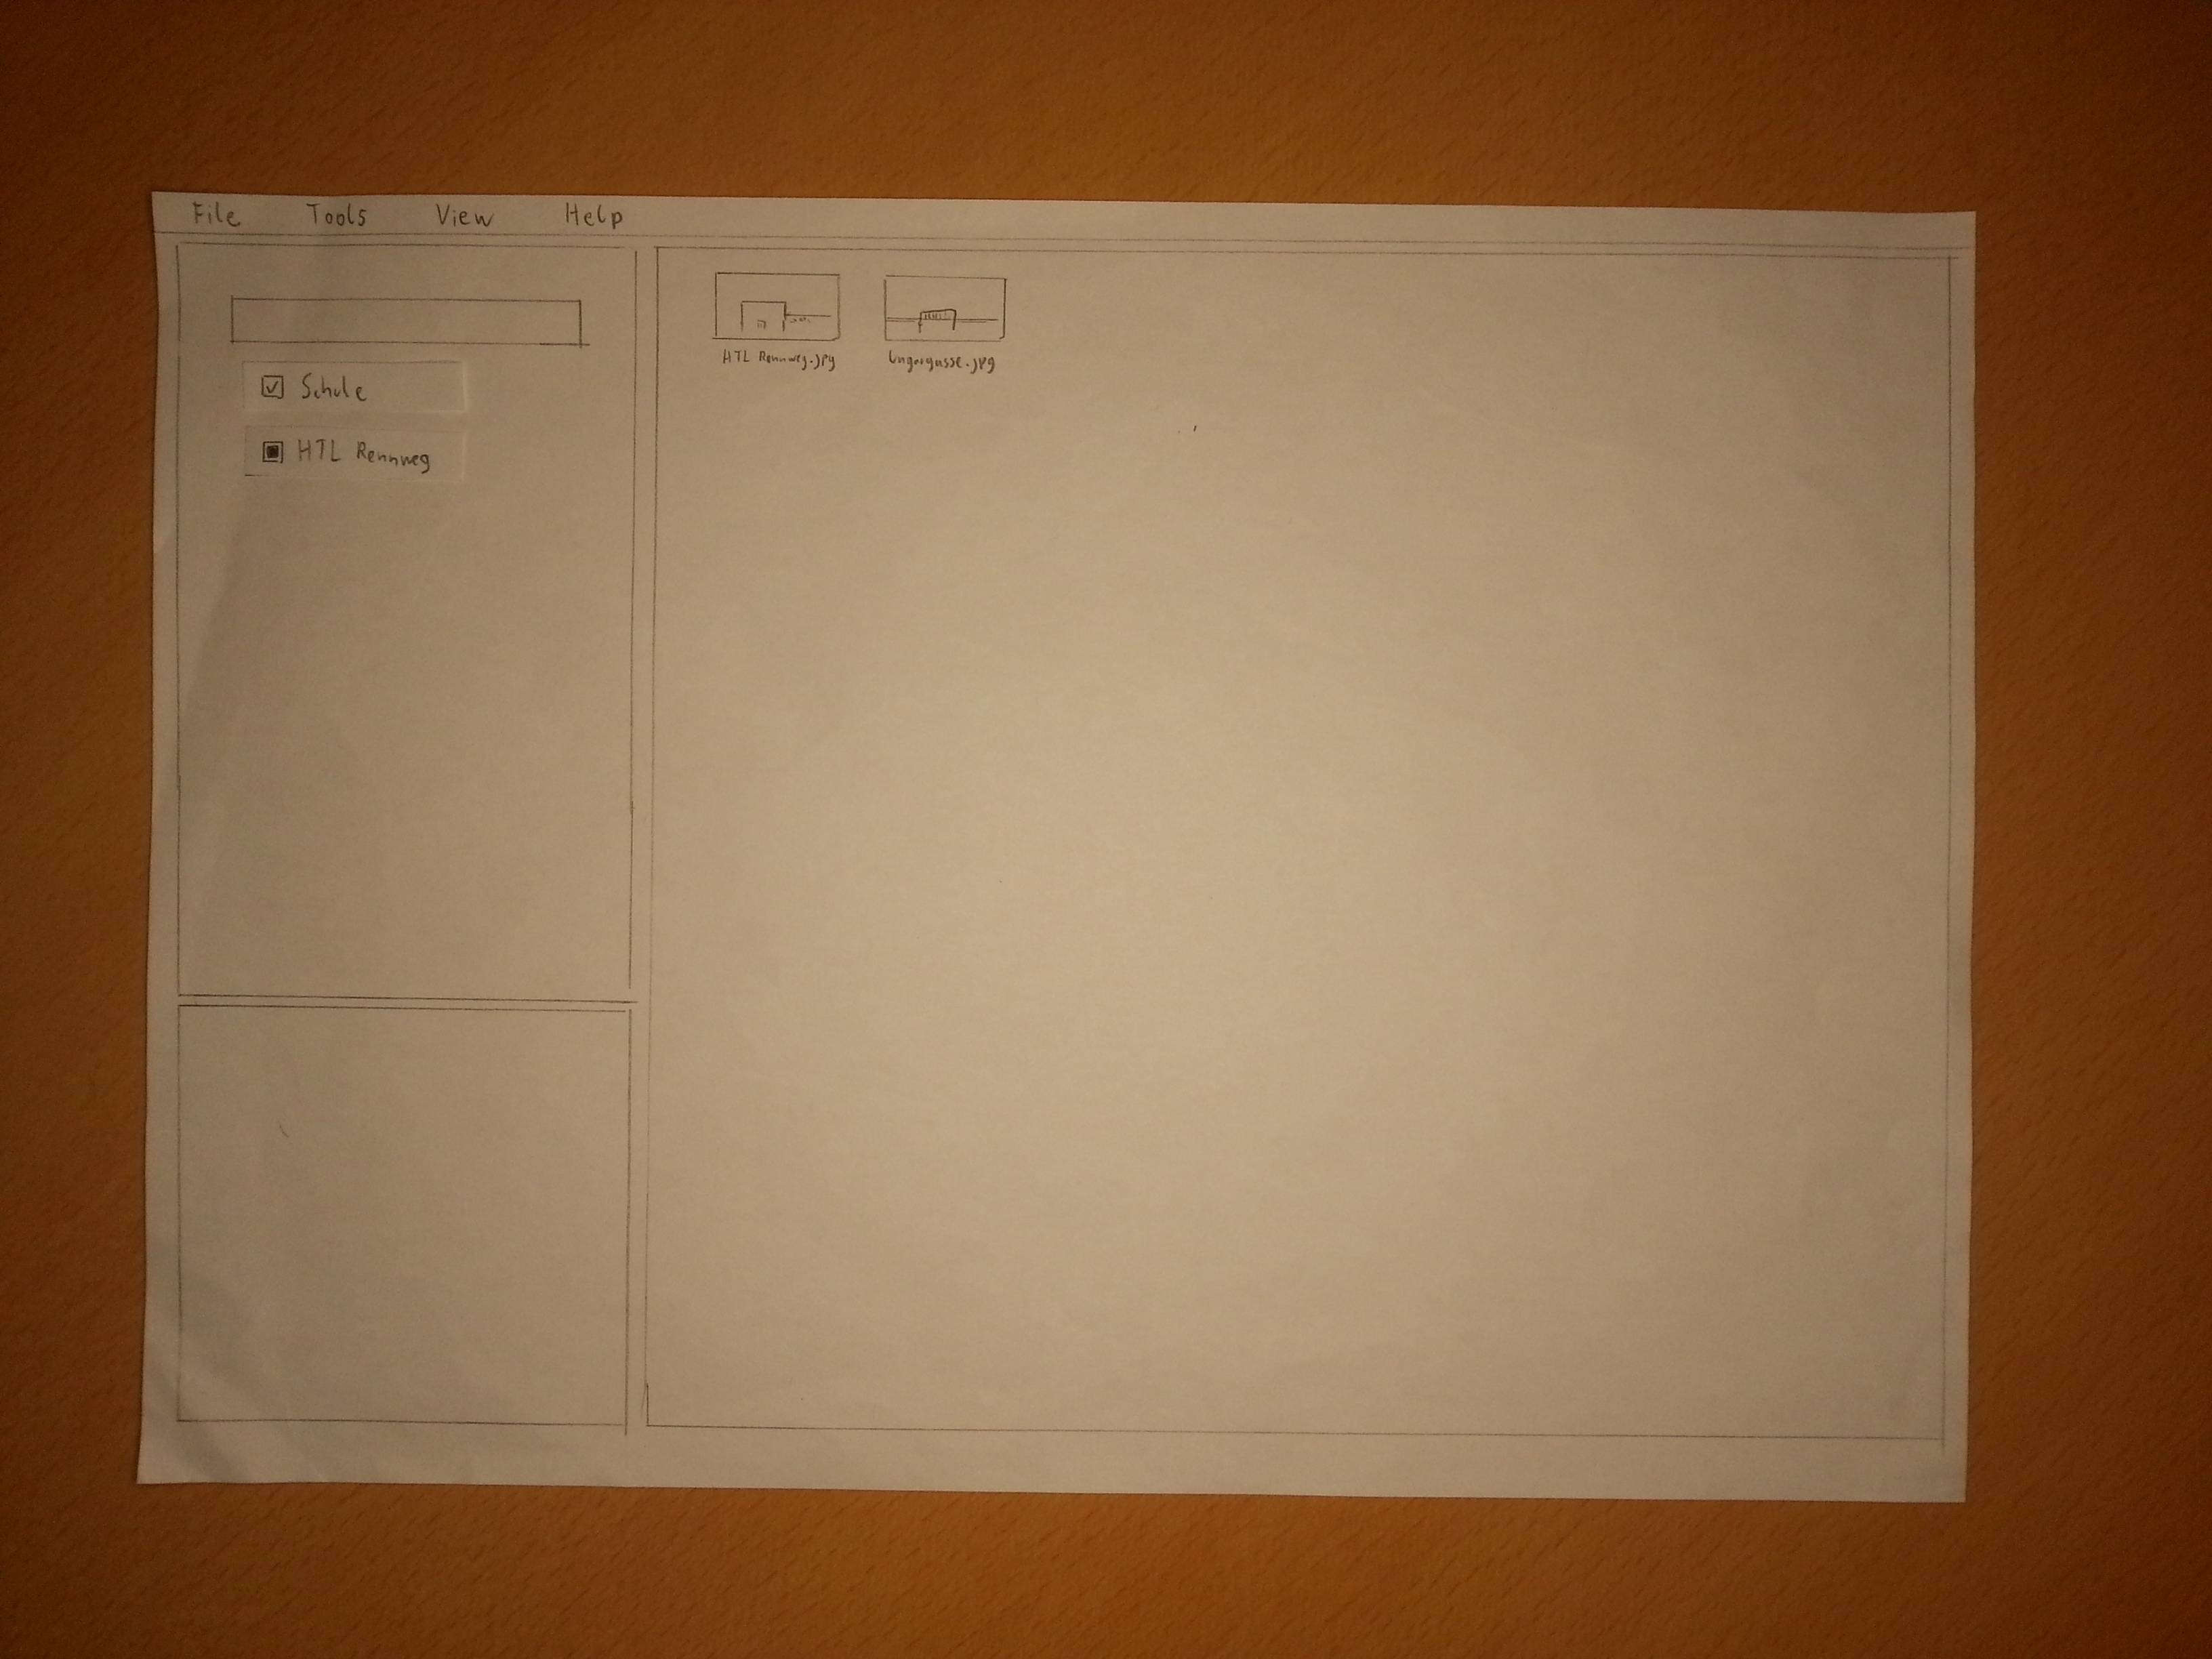
\includegraphics[width=\linewidth]{pp_01}
	\caption{Sketch of the user interface}
\end{figure}

This sketch shows the general structure of the user interface, which is
consistent across every stage and mode of the software. It can be divided into
the following four sections:

\paragraph{Menu bar} This element can be found in almost all desktop
applications. For OctoTagger, four menus were chosen, \emph{File},
\emph{Tools}, \emph{View} and \emph{Help}. The file menu can be used to switch
and create galleries, import files and access the settings. With \emph{Tools}, the
user can start the \emph{tagging mode}, refresh thumbnails, reset or delete the
current gallery, restore all files, and perform a consistency check.  The \emph{View}
menu can be used to access the \emph{folder mode} and to choose, whether all,
tagged, or untagged files should be shown. The \emph{Help} menu can open the \emph{About}
dialog box as well as the user manual.

\paragraph{Main panel} This is the largest area of the user interface. Its content
depends on the current mode. For example, in \emph{overview mode}, the default,
all imported files are displayed. The items can be selected in order to perform
operations on them (such as renaming, deleting, and assigning tags). Selecting
items works the same way as in a standard file manager, so shortcuts
such as Shift+Click and Ctrl+A can be used. % TODO: Style shortcuts

\paragraph{Tag panel} The first element in the top left box is a text field. It
has two different functions: \emph{assigning tags} and \emph{filtering}.  When
one or more files in the main panel is selected, one can enter a tag name in
the text field and press enter. This tag is then assigned to the selected
files, and the tag will be created if it does not already exist. When no files
are selected, the text field can be used to enter \emph{expressions}, such as
``school'' (all files with the tag ``school'') or ``school -htl'' (all items
with the tag ``school'' but without ``htl''). This has the effect that only
items that match the expression are displayed in the main panel.

Below the text field is a list of every tag, with a checkbox and the tag name.
When a file is selected, the corresponding tags are checked. They can be
manually checked and unchecked, in order to add or remove tags. When multiple
files are selected, shared tags are checked, and tags that are assigned to some
but not all of the items are put into the ``third state'', indicating partial
applicability. This state is usually illustrated as a square, but it can depend
on the platform. In the case that no files are currently selected, checking a
tag causes the tag name to be entered into the text field, which leads to the
filtering described above. This also works with multiple tags.

\paragraph{Context panel} The last section is located in the bottom left box.
The context panel includes several buttons for performing different actions,
depending on the context. It can, for example, delete the currently selected
files, or open them in an image viewer. The idea here is that it shows all the
actions that are available in the context menu (which appears with right
clicking the main panel), but makes them much more visible. This way, users are
much more likely to find and use them.

\paragraph{}
Another feature worth mentioning here is the \emph{tagging view} (or
\emph{tagging mode}), pictured below. % TODO better reference to picture

% TODO: Better picture
\begin{figure}[!h]
	\centering
	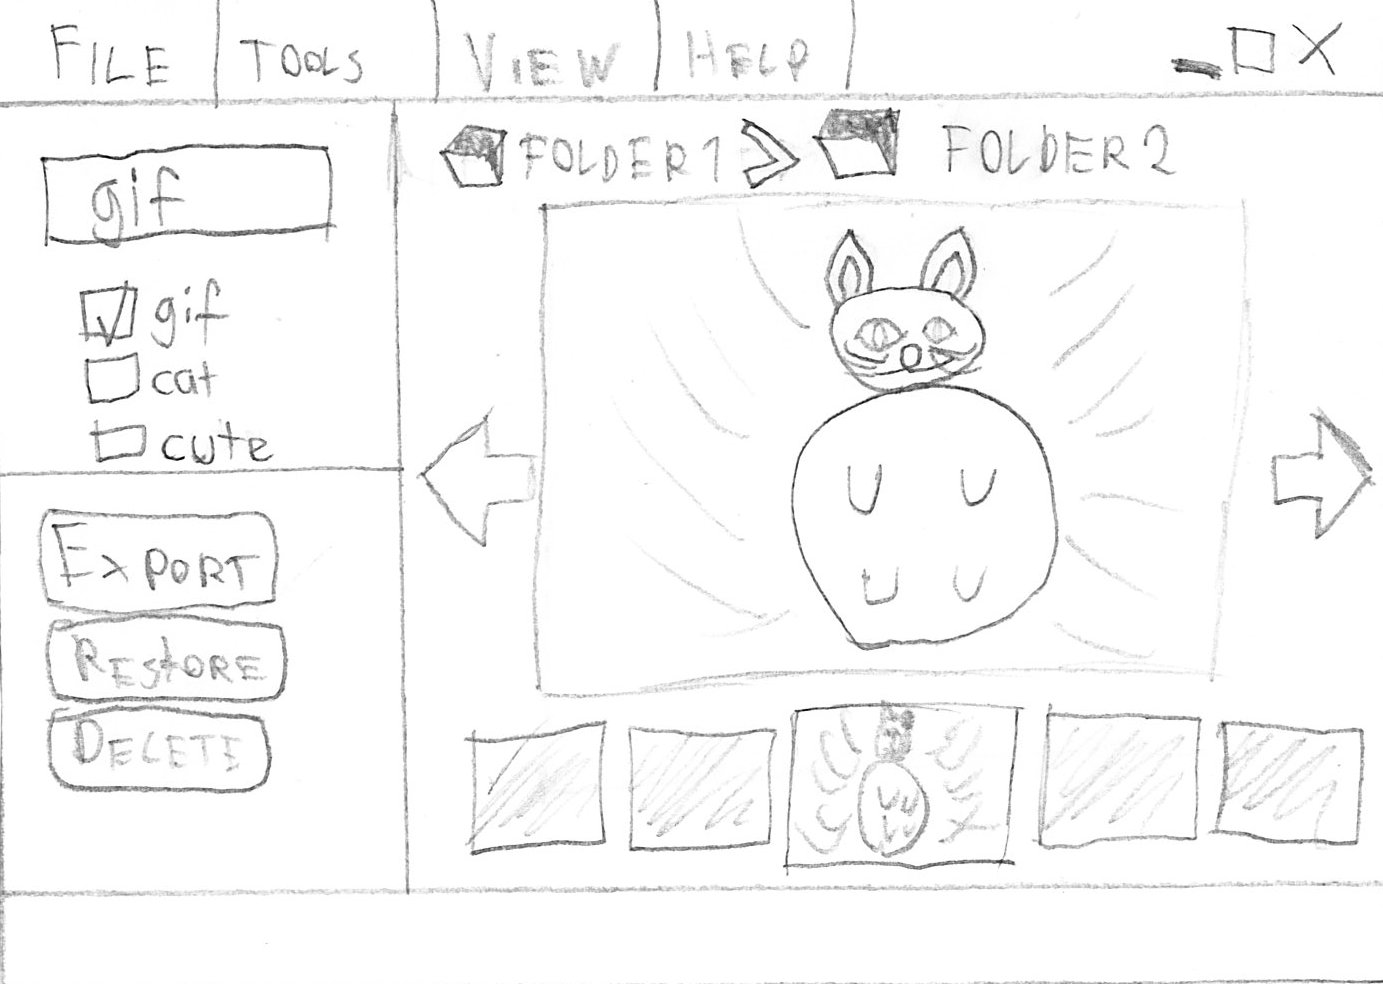
\includegraphics[width=\linewidth]{pp_02}
	\caption{Sketch of the tagging view}
\end{figure}

There are several ways to start this mode. It can be done by double clicking
an item in overview mode, selecting \emph{Start tagging mode} in the
\emph{Tools} menu, or by pressing the according button in the \emph{context pane}.

In this mode, only a single item is visible at a time.
When it is an image file, the image is displayed as big as
possible, and if not, a generic icon is used instead. This mode can be used to
go through a larger collection of photos, look at the content of each one, and
decide which tags apply. The tag and context panes behave the same way as
when a single item in the overview mode is selected.

% TODO chronological order
% function prototypes, learning python
% product backlog
% planning poker
% paper prototype
% code snippets

\section{Structure}
\def\kapitelautor{Clemens Stadlbauer}

In our code repository there are several folders, each of which contains a
certain category of files.

\begin{itemize}
	\item[\tfpath{doc/}] The documentation of the software, i.e.~the user manual
	\item[\tfpath{icons/}] All the different icons and the logo used throughout the software
	\item[\tfpath{db/}] Database schemas and the database setup script
	\item[\tfpath{src/}] The actual code of the software
\end{itemize}

\subsection{Database}

% TODO ER-Model

\tfpath{system.sql} contains the schema of the main database which in turn
contains the user settings and the location of all galleries.
\Cref{lst:db:system} on \cpageref{lst:db:system} shows the entire schema. When
the program is started for the first time these tables are filled with the
following default values.

\begin{table}[!h]
	\centering
	\begin{tabular}{lr}
		\toprule
		\multicolumn{2}{c}{gallery} \\
		\midrule
		\tfcode{name} & \mintinline{sql}{'default'} \\
		\tfcode{location} & \mintinline{sql}{'.'} \\
		\toprule
		\multicolumn{2}{c}{settings} \\
		\midrule
		\tfcode{default_gallery_path} & \mintinline{sql}{'.'} \\
		\tfcode{default_folder_path} & \mintinline{sql}{''} \\
		\tfcode{use_softlink} & \mintinline{sql}{TRUE} \\
		\tfcode{import_copy} & \mintinline{sql}{TRUE} \\
		\tfcode{use_dark_theme} & \mintinline{sql}{TRUE} \\
		\tfcode{current_db} & \mintinline{sql}{TRUE} \\
		\bottomrule
	\end{tabular}
	\caption{Default settings}
\end{table}

Every gallery has its own database as described in \tfpath{gallery.sql}
containing all imported files, all created tags and all created output folders.
The connections between these items (for example which tags a file has) are
recorded in intermediate tables. \Cref{lst:db:gallery} in
\cpageref{lst:db:gallery} shows the entire schema.

Furthermore, the directory contains the helper script \tfpath{setup.py} to
create the initial system database and an empty gallery database which is
copied every time a new gallery is created by the user.

\begin{listing}[!ht]
	\begin{minted}{sql}
		CREATE TABLE gallery (
			pk_id INTEGER PRIMARY KEY AUTOINCREMENT,
			name TEXT,
			location TEXT
		);

		CREATE TABLE settings (
			pk_id INTEGER PRIMARY KEY AUTOINCREMENT,
			default_gallery_path TEXT,
			default_folder_path TEXT,
			use_softlink BOOLEAN,
			import_copy BOOLEAN,
			use_dark_theme BOOLEAN,
			current_db INTEGER REFERENCES gallery(pk_id)
		);
	\end{minted}
	\caption{System database schema}
	\label{lst:db:system}
\end{listing}

\begin{listing}[!ht]
	\begin{minted}{sql}
		CREATE TABLE tag (
			pk_id INTEGER PRIMARY KEY AUTOINCREMENT,
			name text UNIQUE ON CONFLICT ABORT,
			is_numeric BOOLEAN
		);

		CREATE TABLE folder (
			pk_id INTEGER PRIMARY KEY AUTOINCREMENT,
			name TEXT,
			location TEXT,
			expression TEXT,
			use_softlink BOOLEAN
		);

		CREATE TABLE gallery_folder (
			pk_id INTEGER PRIMARY KEY AUTOINCREMENT,
			name TEXT,
			location TEXT,
			add_new_tag BOOLEAN,
			use_softlink BOOLEAN
		);

		CREATE TABLE gallery_folder_has_tag (
			pk_fk_gallery_folder_id INTEGER REFERENCES gallery_folder(pk_id),
			pk_fk_tag_id INTEGER REFERENCES tag(pk_id)
		);

		CREATE TABLE file (
			pk_id INTEGER PRIMARY KEY AUTOINCREMENT,
			uuid TEXT UNIQUE ON CONFLICT ABORT,
			file_name TEXT
		);

		CREATE TABLE file_has_tag (
			pk_fk_file_id INTEGER REFERENCES file(pk_id),
			pk_fk_tag_id INTEGER REFERENCES tags(pk_id),
			amount INTEGER
		);
	\end{minted}
	\caption{Gallery database schema}
	\label{lst:db:gallery}
\end{listing}

\subsection{Source}
Herein lie all the modules that make up the entirety of the functionality and
design of OctoTagger. Each module is contained in a single file with the
module's name and can be categorizes as either frontend or backend. All the
frontend modules provide some part of the user interface while all the backend
modules implement mostly all the functionality that happens in the background
(for example the management of files). The main file is \tfpath{octotagger.py},
which is used to start the program.

% TODO module tree?


\section{Frontend}
%TODO subsection titles as e.g. "Context pane" or "contextpane.py"?

% TODO order
\subsection{\tfcode{octotagger}}
\def\kapitelautor{Erik Ritschl}
%todo wrong author?

This is the main module, the file that needs to be executed in order to start OctoTagger. It consists of the class \tfcode{MainWindow}, which extends
\tfcode{wx.Frame}, which is an application window in wxPython\index{wxPython}.
The code that starts the main loop is located at the very end of the file. %TODO include link
With almost 2000 lines of code, this is the largest source file in the whole
project. The reason for this is that it includes many functions that could not
be easily outsourced as a module, such as three of the four modes (\emph{overview}, \emph{import} and \emph{folder}). Because of the interactive nature of graphical user interfaces, the majority of the  functions consist of event handlers. Given below is a overview of the
module's general structure.

\subsubsection{Starting the software}

This is the very first code that gets executed, and can be found at the end of the file at \tfpath{Source Code/octotagger/src/octotagger.py}:

\begin{listing}[H]
    \begin{minted}{python}
        app = wx.App(False)
        frame = MainWindow(None, "OctoTagger")
        app.MainLoop()
    \end{minted}
    \caption{OctoTagger's main loop}
\end{listing}

It first creates the application object, then the window for it, and finally starts the main loop. The constructor of \tfcode{MainWindow} initializes the basic user interface and sets some variables
used throughout the application, such as the color theme and the current mode.
The mode can be one of four strings: \tfcode{overview} (the default),
\tfcode{tagging}, \tfcode{import}, and \tfcode{folder}. The basic elements are created here. They consist of the menu bar, panels,
sizers (which determine where each element is located and how it reacts to
resizing), and the text field. %TODO mention autocompletion

An \emph{accelerator table} is also created. This is a feature
of wxPython\index{wxPython}, with which one can specify an array of key code
and function pairs, each of which then serves as an \emph{accelerator}, or
keyboard shortcut.

\tfcode{start_overview} is the last function called in the constructor. It sets the current mode
to the default \tfcode{overview}, and gracefully ends any previously active
mode. For example, if it is called during \emph{import} mode, it first asks the users they really want to cancel the import.

In order to start the \emph{overview} mode, a query for all file ID's is made via the
gallery's database. These are then given to the \emph{item view}, which proceeds
with loading the every item. This is where the applications initialization
ends, and control is passed over to the user. 

\subsubsection{Modes and general functions}

%TODO link taglist
The application's modes are not just defined in a few functions or classes, but are rather a conglomerate of 
different behaviors in every element. For example, when a tag gets selected via checkbox in the \emph{tag list}, the function \tfcode{select_tags} is called, which then does different things depending on the \tfcode{self.mode} variable. If its value is \tfcode{"folder"}, the function exits immediately because it should not have any effect in \emph{folder} mode. But in \emph{overview} and \emph{tagging} mode, the selected items get the corresponding tag either assigned or unassigned, depending on the circumstances. But there are also many functions that work only in their specific mode (these are described in following sections) or completely independently from the active mode.

Because a lot of \tfcode{If}-Statements are involved, some convenience functions were created. For example, the way selected items are measured in \emph{tagging} mode differs from the other modes, and that is why a function was written that always returns the currently selected items, regardless of active mode.

\emph{Open gallery} is a submenu of the file menu, under which the user can
select one of the available galleries to open. Since they can change during
runtime, a function had to be written for updating its contents.

\emph{Refresh thumbnails} is an option in the \emph{tools} menu which is also accessible by pressing \emph{F5}. It regenerates all thumbnails of the currently selected files, or of every file when nothing is selected. This is necessary when an image file has been edited and the current thumbnail no longer represents it correctly.

\subsubsection{Overview mode}

%TODO link item view, tag list, context pane, tagging view
In \emph{overview mode}, all imported files are displayed in the \emph{item view}. Selecting items calls \tfcode{on_selection_change}, which then in turn updates the \emph{tag list} accordingly, by checking the relevant tags, and enables the corresponding options in the \emph{context pane} (such as \emph{Rename}, \emph{Open}, etc.). 

Writing into the text field on the top left can have two different results. When no files are selected, it automatically evaluates the input as a tag expression and filters the displayed items by it. Otherwise, it only takes effect when there is a file selection and \emph{Enter} is pressed, upon which the input is interpreted as  a new tag name which then assigned to the items. 

The effect of checking a tag in the \emph{tag list} also depends on whether items are selected. If they are, the tag gets assigned to the items. If not, the tag name is written into the search field, causing the filtering to occur.

The \emph{View} menu has the options to only display tagged, untagged or all files, as well as switching to \emph{folder} mode.

When an item is double clicked, a function gets called that removes the \emph{item view} and replaces it with the \emph{tagging view}. This mode basically behaves the same as \emph{overview}, with exactly one item always selected.

\subsubsection{Folder mode}
When this mode is started by the \tfcode{on_start_folder_mode} function, the \emph{tag list} is completely disabled and the \emph{item view} gets updated, but this time not with file ID's but with the paths of all output folders. In order to tell the \emph{item view} which paths are gallery folders, \tfcode{"|GALLERYFOLDER"} is appended to them. This way, they get listed first and advanced output folders second. Double clicking on a folder icon starts the appropriate editing dialog. They can also be opened in the file manager or removed via the options provided in the context menu and \emph{context pane}.

\subsubsection{Import mode}

This mode is activated by the \emph{Start file import process...} option in the \emph{file} menu. It prompts the user for a directory, which then gets loaded into the \emph{item view}, meaning that the path of all sub-folders and files contained in it are passed over in an array to the \tfcode{ItemView.SetItems} function. Users can then enter sub-directories via double click, and go back to parent folders with the \tfcode{^} button, which is located in the newly added \emph{top bar} above the \emph{item view}.

In \emph{import} mode, tags can be assigned to files that have not yet been actually imported. Therefore, the tag information can not be saved in the database and has to be saved in the object \tfcode{temp_file_tags}, which uses the file paths as keys and tag ID arrays as values. When a file or folder is removed from the import process, its entry in the object is also deleted. Removing items can be very useful when, for example, one wants to import an entire file directory but without one of the sub-folders.

The process can be ended by importing all files, only tagged files, or by aborting. Each of these options is available in the \emph{context pane} and the regular context menu. Since information is lost when aborting, the user is always warned about the consequences when attempting to do so. In all cases, the application returns to \emph{overview} mode.

\subsection{ItemView}
\def\kapitelautor{Clemens Stadlbauer}
\label{subsec:mod:itemview}

\subsubsection{Abstract}
This module lays out a list of items consisting of a thumbnail and a name in a
grid with room to grow off the bottom of the frame. The thumbnails are loaded
in a background thread to make the interface immediately available to the user.

\subsubsection{Attempts}
The original idea was to have a \tfcode{GridSizer} and a rough size for each
item. The number of items per row would have been calculated based on the size
of the containing frame. The problem with this attempt is that quite many
expensive operations and calculations would have to be done on every resize,
potentially resulting in a degraded user experience along with a cluttered
codebase. For this reason a simpler and more elegant solution was searched.

Due to a lack of knowledge on the available \tfcode{Sizers} in
wxPython\index{wxPython} the strategy was to basically try out every one and
analyse it. There always were some problems or limitations with the used
\tfcode{Sizers}, until the \tfcode{WrapSizer} was discovered.

The only problem with this sizer is that it grows off to the right by default
and there seemed to be no way to tell it to grow off the bottom. After trying
to limit the available vertical space of the sizer with no success, it was
placed inside a \tfcode{ScrolledWindow} and after figuring out how to properly
set the size of this window the solution was found.

\subsubsection{Solution} % TODO better title

\begin{sloppypar}
The \tfcode{ItemView} class extends from \tfcode{ScrolledWindow} and is
initialized to vertical scrolling (\tfcode{style=wx.VSCROLL}). Next
two sizers are created, where \tfcode{mainsizer}'s only purpose is to add a
border (\tfcode{wx.EXPAND | wx.LEFT | wx.TOP, border=10}) around
\tfcode{sizer}, which is initialized as a \tfcode{WrapSizer} with horizontal
stacking (\tfcode{wx.WrapSizer(wx.HORIZONTAL)}). Lastly the scroll-rate is set
to roughly half of an \tfcode{Item}'s dimensions for an appropriate scrolling
speed.
\end{sloppypar}

\begin{sloppypar}
The item is a simple panel with a vertical \tfcode{BoxSizer} containing an
image at the top and the name at the bottom. The text is horizontally centered
(\tfcode{wx.ALIGN_CENTER_HORIZONTAL}) and cut off with an ellipsis if it
doesn't fit in the provided horizontal space (\tfcode{wx.ST_NO_AUTORESIZE |
wx.ST_ELLIPSIZE_END}). Event listeners for mouse click events are set up to
delegate them to the \tfcode{ItemView}.
\end{sloppypar}

Upon setting a list of files for \tfcode{ItemView} to display, a number of
steps are taken. First the list is split into several types of files based on
information about each element. If the element is of type \tfcode{int} it
refers to the id of a file in the database. If it is a string it can be an
external file, an external folder or, if the elements begins with
``GALLERYFOLDER'', a gallery folder. Next these sublists are sorted
alphabetically and case insensitive. Lastly they are brought back together in
the order of gallery folders first, then external folders, then external files
and in the end imported files. After all that the new and sorted list is
iterated once again, this time creating a new \tfcode{Item} for each element
with the respective display name, file location and thumbnail.

The number of items displayed during regular use of the program can reach such
a high amount that the loading of the thumbnails can take multiple seconds
degrading the user experience in the process. To resolve this issue all
thumbnails are loaded in the background via the \tfcode{ThumbnailThread} class.
The thread is initialized with the calling window (\tfcode{notify_window}), the
path to the actual image (\tfcode{path}) and the path to the generated
thumbnail or \tfcode{None} if it doesn't exist yet (\tfcode{thumb}).

Once the thread is started it proceeds to generate the thumbnail, if needed,
with thumbnail module (TODO cref). Once it is generated the thread then creates
an \tfcode{Image} from the thumbnail, resizes it to desired size and finally
signals the calling window that the thumbnail has loaded. The calling window,
which is always an \tfcode{Item}, takes the \tfcode{Image}, coverts it into a
\tfcode{Bitmap} and displays it.

\subsection{Tag list}

\subsubsection{Abstract}

This module is responsible for the list of tags on the left side of the window. It sends an event to its parent \tfcode{octotagger.py} when a tag has been checked, it provides functions for checking and unchecking of tags, and it is able to rename or delete tags via rightclick. 

\subsubsection{Attempts}

It was first implemented as an extension of \tfcode{wx.CheckListBox}. It was the easiest way of doing it, since an already finished native module was used, and it mostly provided what was needed: A scrollable list of labeled checkboxes, and plenty of functions for getting and checking items. But a problem soon emerged: the checkboxes in \tfcode{wx.CheckListBox} only support two states, checked and unchecked. But the overview mode requires a third state for indicating partial occurrence of a tag in a selection of files, also called the ``undetermined'' state.

It was then attempted to make a new version of \tfcode{wx.CheckListBox}, by copying and modifying its source code. This turned out to be harder than expected, and was given up on after the realization that crucial know how of wxPython's   internal structure was lacking. Therefore, a completely new class had to be written from scratch.

\subsubsection{Solution}

\tfcode{TagList} is an extension of \tfcode{wx.ScrolledWindow}, which is essentially a panel that receives scroll bars as soon as there is enough content to warrant them. Aside from the standard arguments, its constructor also asks for an array of tag names. Each string receives its own checkbox, this time with the according arguments to make it support three states.

Most of \tfcode{TagList}'s functions are reimplementations of \tfcode{wx.CheckListBox}'s, but there are some novel additions. Rightclicks on an item spawn a context menu, which gives one the option of renaming or deleting the tag. Deletion is very straightforward: First, the appropriate backend functions for properly removing a tag are called, and then an update event is sent to \tfcode{octotagger.py}, which causes a recreation of the \tfcode{TagList} object.

Renaming is a little more complex, and is divided up into two functions. \tfcode{RenameTag} hides the relevant item, replacing it with a text field which contains the tag name. A new name can now be entered. The edit is confirmed with the press of \tfcode{Enter}, upon which the function \tfcode{OnNewName} is called. Here, a check for the validity of the new name is made. An error message is displayed when the name contains anything other than letters, numbers and underscores, or when it is already in use. When the input is OK, the backend function for renaming tags in the \tfcode{output} module is called, after which an update event sent, and the tag list gets redrawn.
\subsection{\tfcode{contextpanel}}
\def\kapitelautor{Erik Ritschl}
\label{subsec:mod:contextpanel}

This panel is located below the tag list, and contains a dynamic list of
buttons for performing various actions. It also extends
\tfcode{wx.ScrolledWindow} \cite{wxScrolledWindow}, which makes it scrollable. The list is updated via
the method \tfcode{SetMode}, which takes the software mode and amount of
selected items (none, single or multiple items) as arguments. Most buttons are
directly bound to functions in \tfcode{octotagger.py} (e.g.
\tfcode{RemoveItem}).

\subsection{\tfcode{settings}}
\def\kapitelautor{Erik Ritschl}

The settings menu, which can be found in the file menu, is a custom dialogue window (\tfcode{wx.Dialogue}) \cite{wxDialogue}, and provides five options to the user. With \emph{Default gallery folder} and \emph{Default folder location} the user can specify specific paths that should automatically be filled in when a gallery folder or advanced output folder is created. \emph{Default linking method} defines whether hardlinks or softlinks are used by default. \emph{Import method} sets whether files are copied or moved during import, and with \emph{Color theme} the user can choose the preferred theme of the user interface, bright or dark.

The implementation is very simple. On load, the current settings are loaded into the input fields, and saving causes the input to be checked for validity and subsequently written into the database.
\subsection{\tfcode{new gallery}}
\def\kapitelautor{Erik Ritschl}

The \emph{New gallery} dialogue can be opened via the file menu, and is used to create a new gallery. Its implementation is very straightforward. It asks for a name and path, and should the input be valid, the appropriate functions in the \tfcode{database} module are called: \tfcode{create_gallery} and \tfcode{switch_gallery}, in order to open it immediately. Should a it have been configured, the specified default gallery path in the settings is written into the folder path input field on creation of the window.
\subsection{Create/Edit output folder}

This section technically covers two modules, \tfcode{create_output_folder} and \tfcode{edit_output_folder}, but they actually are copies of each other with some slight differences. 

When creating an output folder, the user is asked to specify its four attributes, its \emph{name}, \emph{expression}, \emph{location}, and the type of \emph{symbolic link} to be used. Pressing \emph{Ok} causes the folder to be created and registered in the database.

It can be edited by double clicking it in the folder mode. The current settings are filled in automatically, and can be edited and updated. In both scenarios checks for the validity of the input are made. For example, if the expression contains tag names that do not exist, a warning is shown to the user. 

In the first implementation, expressions were simply saved as a strings, just they way the user typed them. But this was not a viable solution once tags could be renamed. One would have had to update every expression in all folders containing a recently renamed tag. This issue was solved by first converting the expression string to not use the names, but IDs of the tags. When reading an expression from the database, it is converted back. The \tfcode{expression} module also had to be updated to accommodate this change. 

In the case that a tag that was used in an expression is deleted from the system, its name is replaced with question marks within the expression field of the relevant folders, and the user is asked to update it accordingly.
\subsection{Create/Edit gallery folder}

Just like with the output folders, this section combines two modules for creating and editing gallery folders.

The dialog for gallery folders is a little more complex. Besides the name, location and symlink type, it provides options for the contents. There is a check box list with every tag in the system, which controls the tags that should be represented within the folder. So, for example, one can choose to receive a folder for every tag except a few, a kind of blacklist. If the user wants to choose a kind of white list approach, this can be done by disabling the checkbox \emph{Automatically add new tags}. This way, when a new tag is added to the gallery, it will not be automatically enabled on the list, which is otherwise the default behavior.


\section{Backend}

% TODO order
\subsection{\tfcode{database}}
\def\kapitelautor{Erik Ritschl}

This module provides several functions for dealing with the various database
files in OctoTagger. It is responsible for creating, switching, resetting
(removing all tags) and deleting galleries. Probably the most used function is
\tfcode{get_current_gallery}. When calling it, one can specify a certain
property, such as ``name'', ``location'' or ``connection'', and it is returned.
This method is used every time the contents of the currently active gallery
database file need to be read or modified at any point in the software.

\subsection{import\_files}

This is the backend module for importing files into the currently active gallery, but it also contains some frontend elements.

It only has a single function, \tfcode{import\_files}, which takes either a list of file paths or a python dictionary, where file paths are the keys and lists of tags the values, as its argument. The former option corresponds to a ``Direct file import'', and the latter to an import via the more complex and powerful import mode.

In both cases, the given data the is being iterated over, and a number of procedures are executed for each file. First, a check is made to ensure that the file actually exists. Then, a random unique ID gets generated, in form of an UUID. The file is then either moved or copied (a preference which can be set in the settings) to the \tfcode{files} folder in the gallery, using the UUID as its name. This is necessary to avoid name conflicts, since all files are located in the same directory. Finally, an entry is made in the database, saving the file's UUID as well as its original name. When a dictionary with tags was passed over, the tag relations are also made here.

As mentioned earlier, there are also some frontend elements. These consist of pop ups that inform the user of any errors that occurred during the import, as well as a progress bar which shows how many files have yet to be imported. There is also an informational pop up at the end that warns the user about any files that have the same name. Same name files supported by OctoTagger in principal, but there are some not easily avoidable inconsistencies that come with them. It was therefore decided to warn the user about the potential issues and urging him or her to change the file names.
\subsection{tagging}

This is one of the most important backend modules. It is this file that provides the necessary functions for creating, assigning, and reading of tags, among others. \tfcode{create_tag} takes a tag name as argument, checks if a tag with that name already exists, writes the tag into the database, and returns its ID. \tfcode{tag_file} takes a file id in addition to a tag name, and writes the relationship to the database, creating the tag in the process should it not already exist. 

The module also provides the means to find out what tags a given file already has or what all registered tags in the system are, converting between ID and name of files and tags, as well as removing tags from files.

% TODO Not well written
\subsection{\tfcode{thumbnail}}
\label{sub:mod:thumbnail}
\def\kapitelautor{Clemens Stadlbauer}

\subsubsection{Abstract}

This module keeps a register that maps mime-types to static images or file
handlers that generate the thumbnails. By default, only jpeg, png and gif
images are handled with a generic handler utilizing \tfcode{PIL}\index{PIL} to
load, size, scale and finally save the generated thumbnail as a png image. If
an image has an unregistered mime-type a generic thumbnail will be used.

\subsubsection{Attempts}

At first we used the original images but it quickly became apparent that this
wasn't the final solution as the interface would hang for multiple seconds on
large images. It was then decided to generate thumbnails of a fixed size and
save them on disk to improve loading times.

\subsubsection{Solution} % TODO better title

The modules has two functions, one for registering new handlers and another for
generating thumbnails.

The first, called \tfcode{register}, takes a mime-type and a handler. It first
checks whether a handler for the specified mime-type already exists, then if
the provided handler is either a valid path or a function. If both checks pass
it registers the new handler.

To actually generate the thumbnail the modules provides the
\tfcode{get_thumbnail} method which takes either a file id from the database or
a path. It then proceeds to check if a thumbnail has previously been generated.
If none was found it tries to generate a new one by first finding the
appropriate handler from the file's mime-type. If the handler is a static image
its path is returned, if it is a function, however, it is invoked with the
file's path and the desired thumbnail's path. The newly generated thumbnail is
then returned.

In addition three default handlers are registered for the \tfcode{image/jpeg},
\tfcode{image/png} and \tfcode{image/gif} mime-types as these are the most
common image types. The generic handler uses the \emph{Python Image
Library}\index{PIL} to load the original image, resize it to fit the desired
size, add padding to exactly fit this size and finally save it as a png file.
While jpeg would provide a smaller file size, it does not support transparency.

To see how and when this modules is used see \cref{subsec:mod:itemview}.

\subsection{\tfcode{expression}}
\def\kapitelautor{Clemens Stadlbauer}
\label{subsec:mod:expression}

\subsubsection{Abstract}

This module's job is to convert an expression (see
\cref{subsec:theory:expression}) to its corresponding SQL query. It does this by
first splitting the expression into segments with Python's \tfcode{Scanner}
\cite{scanner} and then iterating over the segments ensuring syntactical
correctness and building the query in the process.

\subsubsection{Attempts}

Although they weren't multiple attempts during the implementation, there were
during planning.

The first idea was to represent an expression with special datatypes for each
possible token and combinations and groupings between tokens. While this would
have been the most expressive and structured solution it is sadly not possible
to implement in Python because Python has no support for annotated values due
to its lacking type system.

To circumvent this, an alternative solution would be to express values as a
list or dictionary carrying the annotation. The problem with this approach is
that the resulting structure would be nested far deeper than the original
expression and working with it would be needlessly complicated.

\subsubsection{Solution} % TODO better title

Shortly prior to implementing this module, Clemens, who was responsible for the
implementation, read about an undocumented feature inside Python's \tfcode{re}
module that provided exactly the functionality needed for the first step.
\tfcode{Scanner} is the class in question and it works by splitting a string
into parts based on a list of regular expressions and optionally passing the
part through a conversion function. For OctoTagger the parts don't need to be
converted but this feature is used to strip whitespace and error on unknown
tokens.

\begin{listing}[H]
    \begin{minted}{python}
        scanner = re.Scanner([
            (REG_NUM, identity),
            (REG_TAG, identity),
            (REG_OP, identity),
            (REG_GROUP, identity),
            (r'\s+', None),
            (r'', unknown),
        ])
    \end{minted}
    \caption{Expression token scanner}
\end{listing}

After a simple parenthesis count the tokens are step by step grouped together.
First the three tokens required for the numerical comparison (tag name, literal
``='' and number) are grouped into one token. Next all completed comparisons
are converted to a query and then, if present, inversions (read ``not'') are
applied.

At this point all comparisons are finished and only need to be combined. This
happens by first grouping together all tokens inside a group (enclosed by
parentheses). The last step is to split the tokens at ``or'' tokens (``/''),
pairing the tags within both sides with ``and'' and finally pairing the sides
with ``or''.

\paragraph{Additional methods}

In addition to converting an expression to a query, this module also provides
two methods to map over tag names or ids inside an expression named
\tfcode{map_tag_name} and \tfcode{map_tag_id} respectively. What these
functions do is pass each tag name or id to a supplied callback function and
use the result of the callback as a replacement.

These functions are mainly used for converting an expression with tag names,
which the user enters, to an expression with tag ids, which is stored in the
database, and converting the other way.
% TODO cref where it is used?

\subsection{output}
\def\kapitelautor{Clemens Stadlbauer}

\subsubsection{Abstract}

This module provides a multitude of methods for changing output folders.
Functionality spans from renaming a folder over changing the link type (TODO
cref to explanation) to handling file tag changes.

\subsubsection{Solution} % TODO better title

Every method has the same basic procedure. First, a list of all affected output
folders is acquired, then for each folder the current status is analysed and
finally the required changes are performed.

% TODO maybe go into detail how foreign files are handled?

\paragraph{Output folder placement}

is controlled with the \tfcode{move} and \tfcode{rename} methods that move or
rename an output folder, respectively.

\paragraph{Output folder structure} % TODO better title

is controlled with one of three methods. The first is \tfcode{change_link_type}
which switches an output folder from softlinks to hardlinks or vice versa. This
is the only method in this category that is applicable to both gallery output
folders and advanced output folders.

Specific to gallery output folders is \tfcode{change_gallery} which changes
the list of tags to be contained in the folder. Specific to advanced output
folders, however, is \tfcode{change_expression} which, as the name says,
changes the expression for the folder.

\paragraph{Output folders}

in general are handled by \tfcode{create_gallery}, \tfcode{delete_gallery} and
\tfcode{delete_folder}. The first is used to create the necessary folder
structure for gallery folders, while the latter are used to clean up output
folders requested to be deleted.

\paragraph{Files}

have many methods for editing. There is the simple
\tfcode{change} to assign or remove a tag from a file. Then there are
\tfcode{rename_file} and \tfcode{rename_tag} to change the displayed names of
existing files or tags. Finally, for removal, \tfcode{remove} and
\tfcode{delete_tag} are provided to delete files or tags, respectively.

\subsection{\tfcode{integrity}}
\def\kapitelautor{Clemens Stadlbauer}

\subsubsection{Abstract}

This modules checks if a gallery's database became out of sync with the file
system at some point. The \tfcode{check} method updates all output folders and
informs the user of missing or extra files in the gallery.

\subsubsection{Attempts}

Early during development, even before gallery output folders existed, an
incomplete version of the integrity check existed which only updated output
folders. Development was moved to other, more important parts of OctoTagger
until towards the end of development this module was completely redone with all
the new features in mind.

\subsubsection{Solution} % TODO better title

The functionality can be split into three parts: gallery output folders,
advanced output folders and the gallery source folder. For all output folders
missing files are created. Gallery output folders have the additional check if
folders for each associated tag are present.

The gallery source folders are handled more carefully because the user is
expected not to interact with it meaning discrepancies could be the result of
an unknown error from the user. Because of this no files are modified or
deleted, instead the user is informed.

% TODO screenshot


% TODO explain code
% each module has a small abstract explaining what and how it works
% each module explained roughly in chronological order

\section{User manual}

\section{Corporate Design}
%\subsection{Corporate Identity}

What is the first thing you should think about, when you see our logo? Why did we use these colors? Why did we decide to take this font? 

These are just a few questions related to the corporate identity. It determinates how the project team presents itself to the public. Within the corporate identity document everything regarding public appearance can be defined. This could contain the behaviour to the public, as well as communication, philosophy, design, language and much more. 

In case of OctoTagger it was decided to just take care of the design part from the corporate identity, the corporate design. This document contains our design-guidelines for the website. This includes the colors used for the logo and other images, the background colors, the font and the logo itself. 

The challenge at developing a corporate design is to always keep the user in mind. How does the user think? What does he want to see? It's important to attract a potential user and catch his attention. The website is the first thing every potential user gets confronted with, so it has to send the right signals. Colors are great triggers for emotions and feelings making them a powerful tool for the writer of the corporate design. However, the proper combination of the colors is at least as important as the colors themselves. 

The logo design should not be neglected. It's an essential part of the corporate design. The challenge is to design a logo that provides a distinctive look but keeping it as simple as possible at the same time. 

\subsection{Background of the name OctoTagger}

In the beginning there was just the idea for the product, an file organisation software. Afterwards the name OctoTagger was born. The intention behind that name was indeed an octopus and it's ability to handle several actions at the same time, due to his eight arms. In this point OctoTagger and octopuses share similarities. OctoTagger is also able to handle multiple files at the same time. So the octopus became our mascot and the corporate design was developed out of this idea later. 

\subsection{Corporate Design for OctoTagger}
\subsubsection{Colors}

The colors were the first part of the corporate design to be defined. Because of our mascot the octopus, it was decided to chose colors related to the living environment of octopuses which is the sea. We picked several shades of green and blue to fit this scheme. These tones became our primary colors which means that they are used most of the time. However, just using this colors would be too monotonous, so a secondary color set was added. It contains some complementary colors of the primary colors and is just used rarely.

\paragraph{Primary Colors} \hspace{0pt} \\

\definecolor{primary_1}{RGB}{118,178,76}
\definecolor{primary_2}{RGB}{49,201,175}
\definecolor{primary_5}{RGB}{130,227,166}
\definecolor{primary_3}{RGB}{23,197,200}
\definecolor{primary_6}{RGB}{123,215,213}
\definecolor{primary_4}{RGB}{59,177,216}

\begin{tabular}{ c  c  c  c }
\#76B24C & \crule[primary_1]{3cm}{3cm} & \#31C9AF & \crule[primary_2]{3cm}{3cm} \\
\#17BBC8 & \crule[primary_3]{3cm}{3cm} & \#3BB1D8 & \crule[primary_4]{3cm}{3cm} \\
\#82E3A6 & \crule[primary_5]{3cm}{3cm} & \#7BD7D5 & \crule[primary_6]{3cm}{3cm} \\ 
\end{tabular}

\paragraph{Secondary Colors} \hspace{0pt} \\

\definecolor{secondary_1}{RGB}{255,193,0}
\definecolor{secondary_2}{RGB}{255,140,62}
\definecolor{secondary_3}{RGB}{255,92,62}

\begin{tabular}{ c  c  c  c }
\#FFC100 & \crule[secondary_1]{3cm}{3cm} & \#FF8C3E & \crule[secondary_2]{3cm}{3cm} \\
\#FF5C3E & \crule[secondary_3]{3cm}{3cm} \\
\end{tabular}

\paragraph{Background Colors} \hspace{0pt} \\

\definecolor{background_1}{RGB}{240,240,240}
\definecolor{background_2}{RGB}{193,200,197}

\begin{tabular}{ c  c }
\#F0F0F0 & \crule[background_1]{6cm}{3cm} \\
\#C1C8C5 & \crule[background_2]{6cm}{3cm} \\
\end{tabular}\\



During the color-planing process it was decided to include two different background colors into the corporate design. The first one is a light gray shade which reduces the contrast between the background and the content above it. It is used as background color on the entire website. The second color consists of a much darker shade of gray. It's mainly used to create a second background layer over the first background. 

\subsubsection{Fonts}

As font, the DejaVu font family is used on the website. It follows the general guidelines of the OctoTagger website by being straight and modern. Below an example of the DejaVu font can be seen.\\

\begin{center}
	
\includegraphics[width=\linewidth]{images/font.png}
\end{center}

\subsubsection{Logo}

\paragraph{First drafts} \hspace{0pt} \\

The first concept for the logo of OctoTagger was the combination of an octopus and a folder symbol. These two elements were brought together seamlessly. However, it did not measure up to our expectations as the octopus was hardly recognizable. 

The sketch can be seen in the following image:

\begin{center}
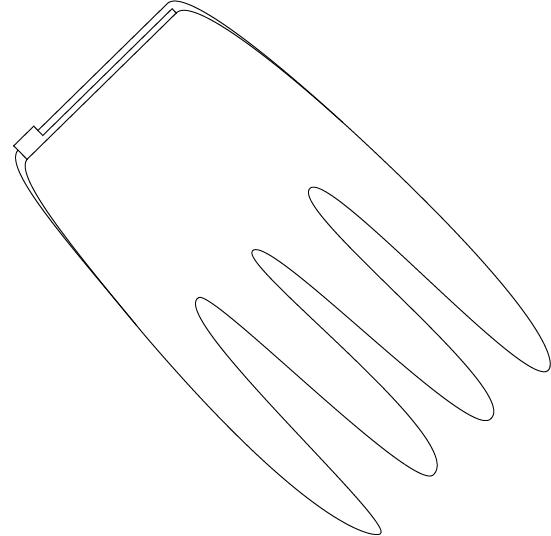
\includegraphics[scale=0.30]{images/logo_v01.png}
\end{center}

The second draft was an enhanced version of the first one. It was tried to keep it more even and linear, furthermore colors were added for the first time. This version of the logo consists of two parts, the file symbol on the top, symbolizing the body of the octopus, and four tentacles below it.

The image below shows the second sketch:

\begin{center}

\includegraphics[scale=0.30]{images/logo_v02.png}
\end{center}

This sketch became even more abstract then the first one and we got some negative feedback. Later it was replaced by an improved version, our actual logo.

\subsubsection{Current logo}

For the final version of the logo, the first concept was adopted and the idea of a folder symbol in our logo was dropped. It was decided to just include the octopus into the logo. This octopus has four visible tentacles on the front and four more in the background. At the end of these arms tags are attached.

The outcome can be seen below:


\begin{center}
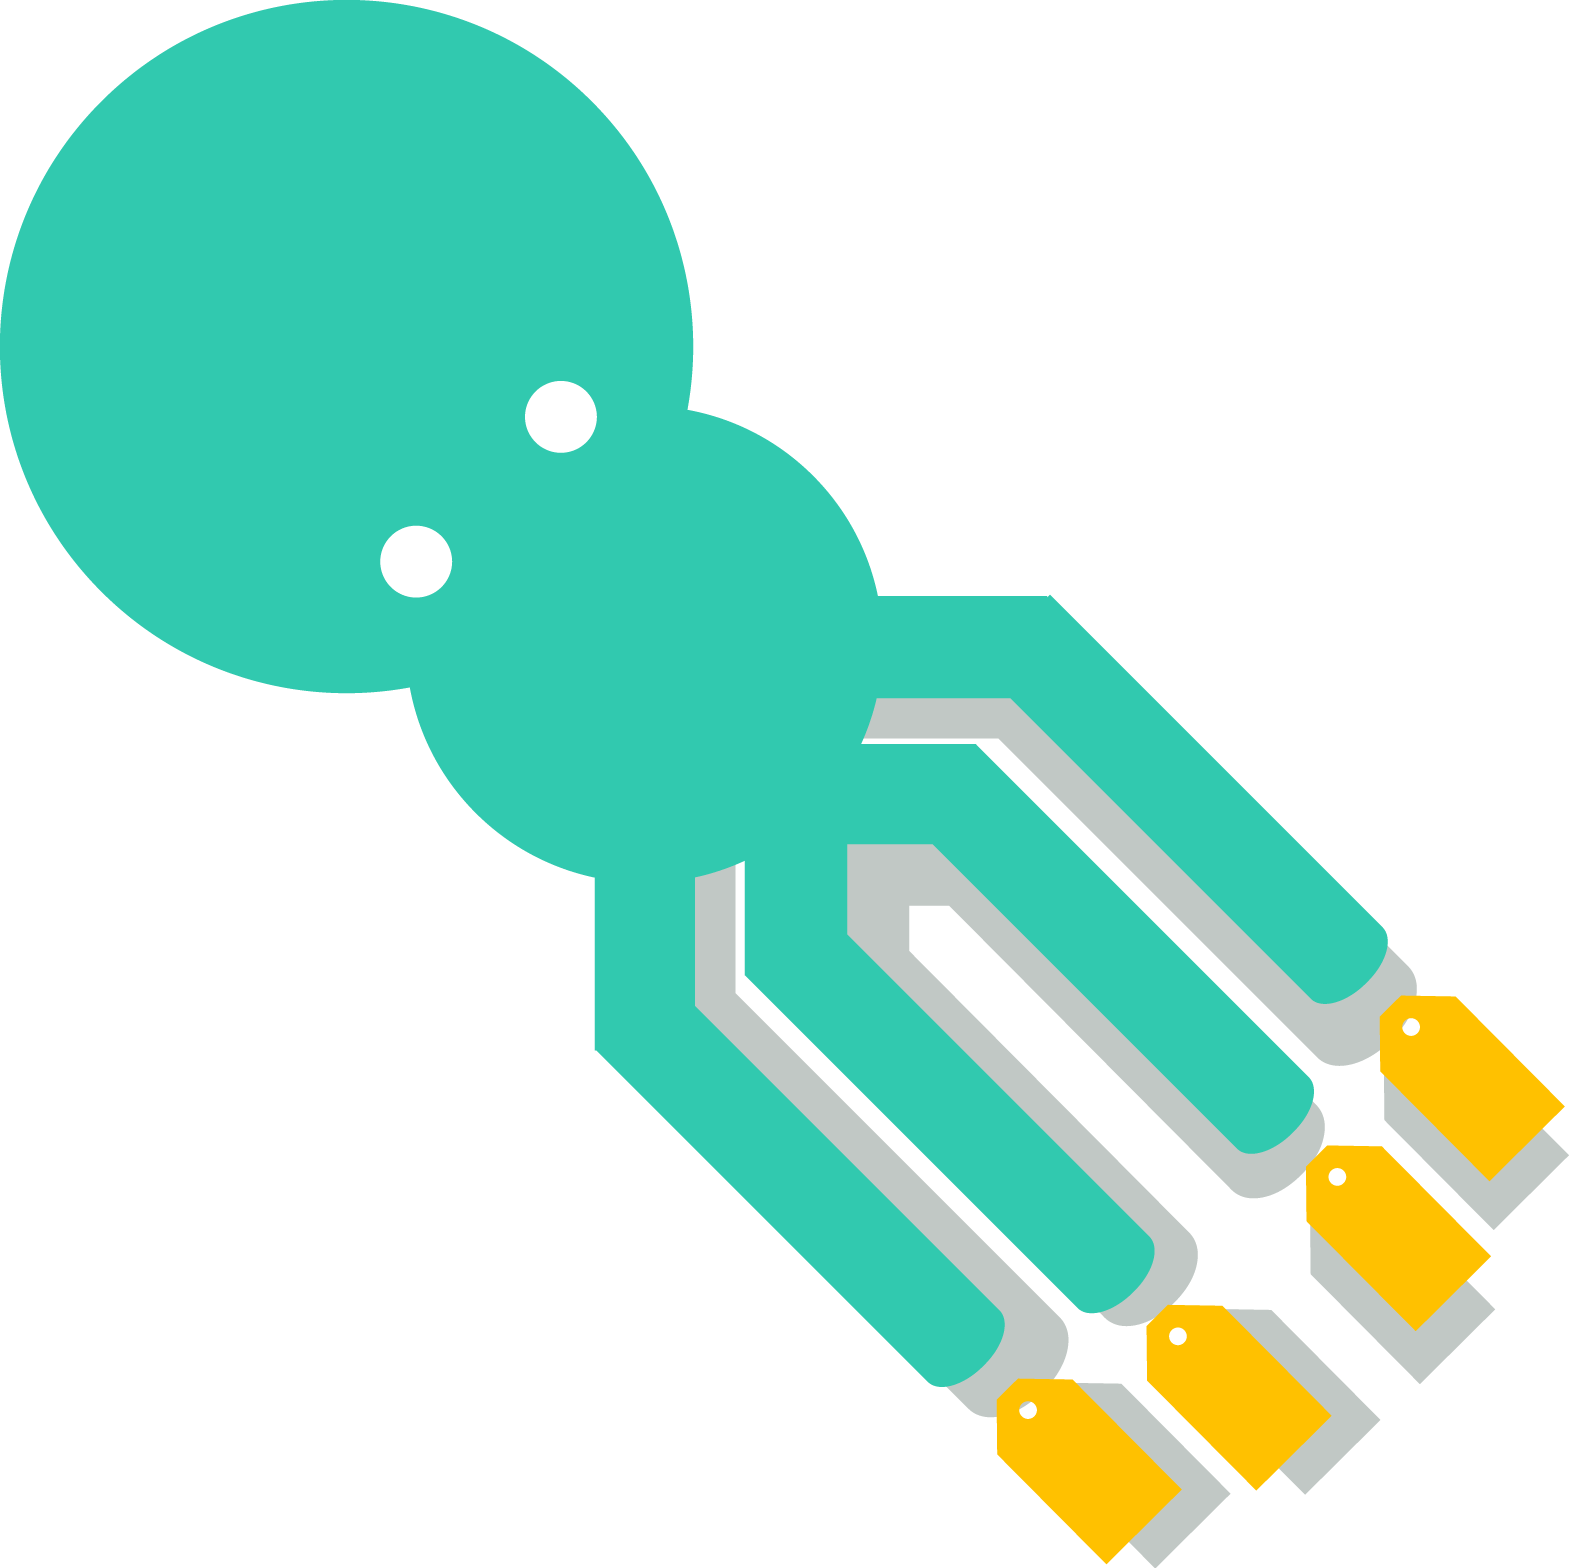
\includegraphics[width=0.5\linewidth]{images/logo.png}

A version including the project name is also available:

\includegraphics[width=\linewidth]{images/logo_text.png}
\end{center}
% TODO message -> colors
\section{Website}
%\subsection{Why is a website important?}

A website is the most efficient way to represent the product as well as the project team. In case of OctoTagger the website also fulfils the task to distribute the product by offering a download. As web developer it's necessary to keep the target audience in mind and adjust the website to its needs.

\subsection{Concept of OctoTagger website}

The website of OctoTagger follows simple and decent design guidelines. It was designed to satisfy the users needs and being as lightweight as possible at the same time. Only few and small images are used on the entire site keeping loading times short.

A major aspect of the website is the ultra-lightweight, straight and modern design. The image design was kept clear and simple without the use of explicit borders. Due to that images appear flat and homogeneous.

\subsubsection{Usability}

The site was developed to be intuitive and easy to use. The user can reach every page independent of his current position.

To make navigation easier, clickable items were made as distinctive as possible. Only buttons and elements of the navigation bar respond to mouse clicks. These objects are also the only ones to respond to hovering, so the user gets signalled that after a click an action will be performed.

As an example for usability, downloading Octotagger could hardly be easier. Every button leading to a download, is colored in a shade of green, compared to other buttons colored in a shade of blue. In fact the user just has to click every green button, follow some installation instructions and is able to use Octotagger after a few minutes.

\subsubsection{Responsive Design}

The challenge for web development is to create a website, that looks good on every available screen size and device like desktop PCs, tablets, phablets and mobile phones. This can be ensured through different solutions.

The first option is to write different CSS sheets for every screen size or device, which requires the most work.

An easier possibility is called responsive design and there are numerous frameworks to support the developer with it. 

Responsive design means that a website is created to work on every device and adapts its appearance based on the screen size and orientation. The concept is based on flexible grids and layouts and the use of CSS media queries.

The following images show the OctoTagger website adapted to different screen sizes:

\begin{center}
\begin{tabular}{ c  c c }
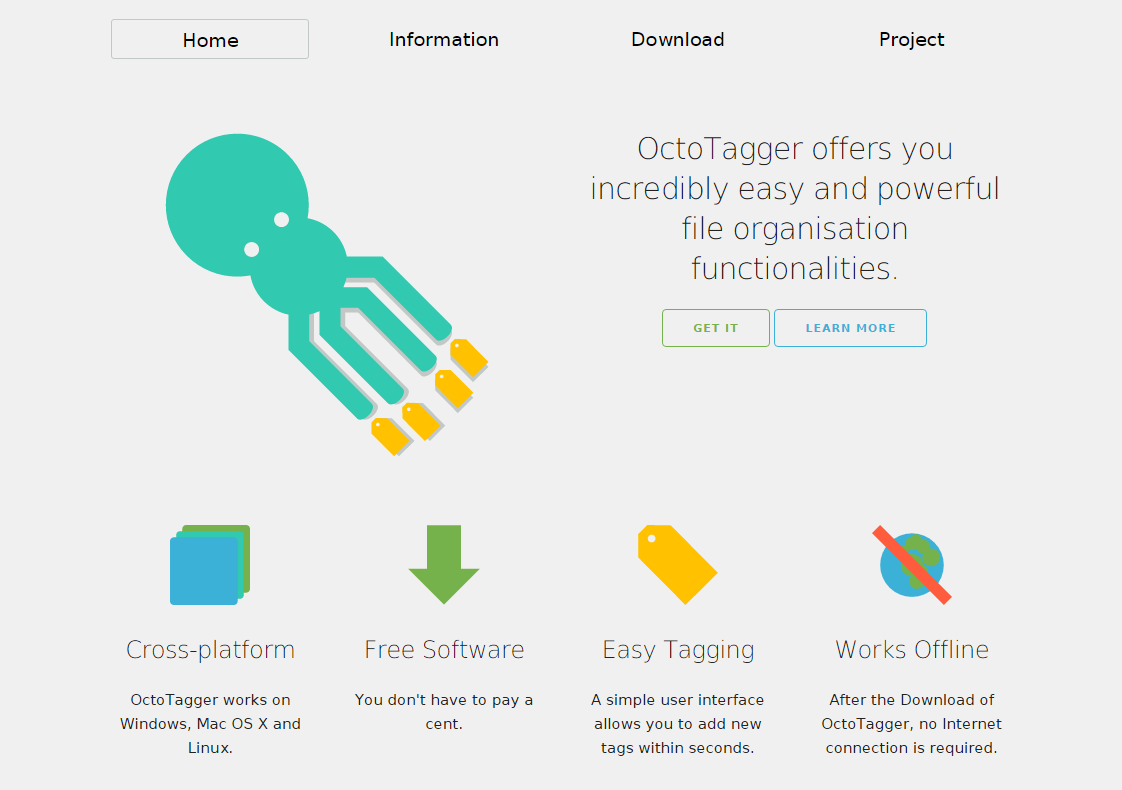
\includegraphics[scale=0.20]{images/home_full.png} & 
\includegraphics[scale=0.30]{images/resize.png} & 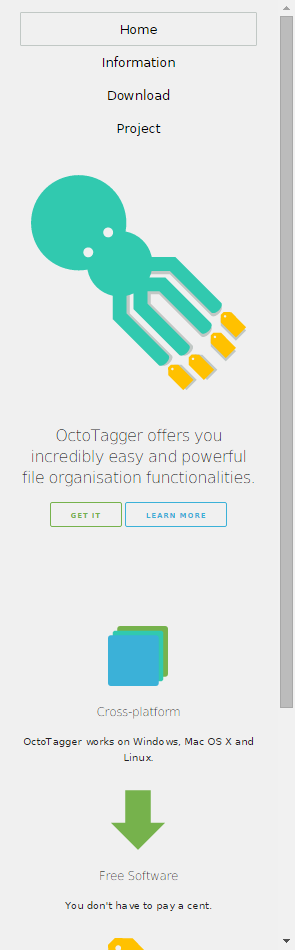
\includegraphics[scale=0.30]{images/home_small.png} \\
\end{tabular}
\end{center}

When the website passes a threshold during the resize, the elements are positioned above each other to fit the smaller screen width. The framework (see \ref{sec:Skeleton}) stacked the elements automatically, but adjustments were still necessary. Some media queries (see \ref{sec:MediaQueries}) had to be adapted so that elements fit perfectly together.

\paragraph{Flexible Grid} \hspace{0pt} \\

Most responsive framework rely on a flexible grid system, with typically 12 columns. Elements in the HTML code can now be positioned within this grid with the help of CSS classes. Depending on the width you want a HTML object to have, you have to give the proper CSS classes.

The image below shows a flexible grid example using the Skeleton framework (see \ref{sec:Skeleton})

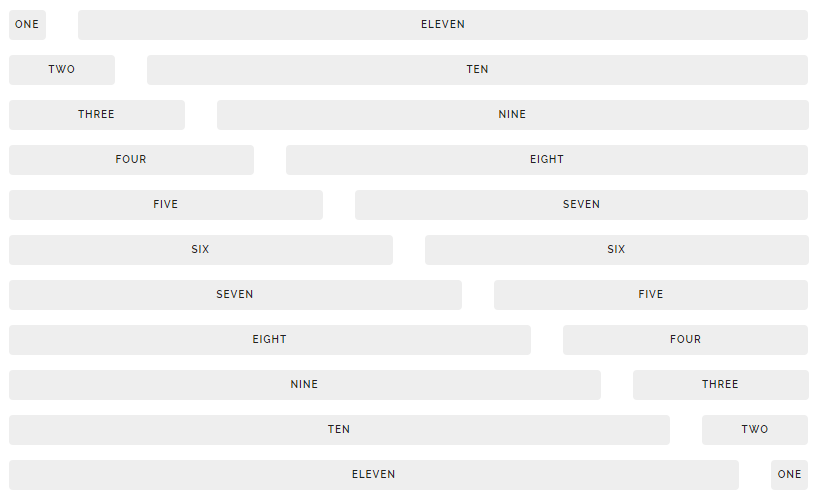
\includegraphics[scale=0.50]{images/skeleton_grid.png} 

\paragraph{CSS Media Queries} \hspace{0pt} \\
\label{sec:MediaQueries}

With the help of CSS Media Queries it's possible to set CSS attributes depending on conditions like screen width and device type. For instance the width of a box can  be increased when the window is enlarged.

The following code snippet shows an example for some width dependant media queries.

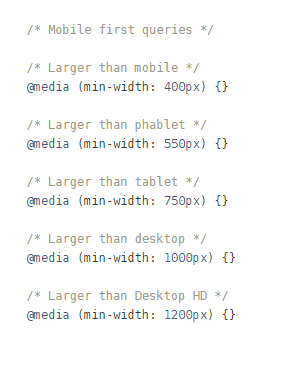
\includegraphics[scale=0.70]{images/media_query.png} 

\subsection{Structure}

The OctoTagger website is basically made up of four pages called Home, Information, Download and Project. All these pages are accessible via the navigation bar which is positioned on the top on every page. In addition there are several sub-pages only accessible on the download site.

\subsubsection{Home page}

\begin{center}
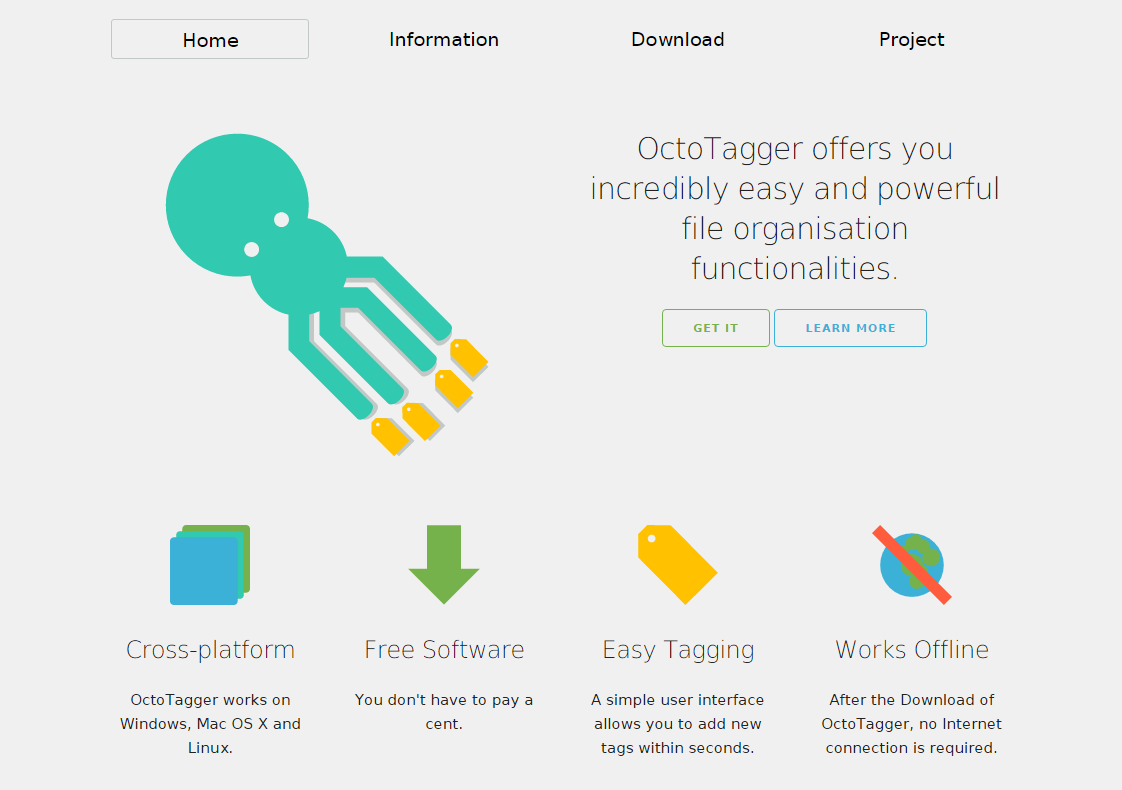
\includegraphics[scale=0.35]{images/home_full.png}\\
\end{center}

The home page is the first thing a user sees when he visits octotagger.co. This page is designed to catch the users attention with the help of a catchy slogan. The button "Learn more" is linked to the information page and with the help of the button "Get it" the user gets transferred to the download page. By just hovering the "Get it" button, a drop down menu appears and offers the possibility to directly download OctoTagger for the users operating system (see \ref{sec:OSdetection}). This option just makes sense, when the user has already installed the required software, of course.

In the bottom part the highlights of the software are pointed out with pictograms and short descriptions. The goal is to show the user the advantages of the software in one glance.

\subsubsection{Information page}

\begin{center}
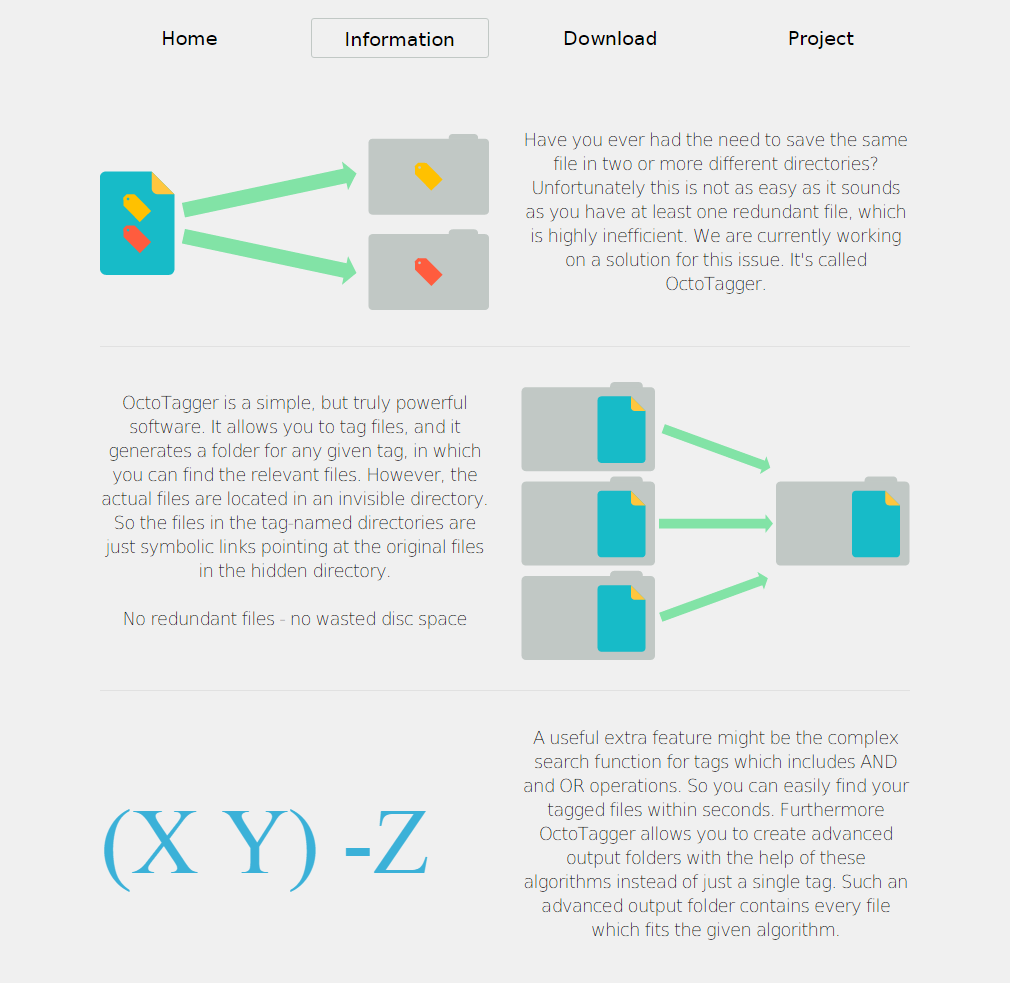
\includegraphics[scale=0.35]{images/information_full.png}
\end{center}

The information page offers the user some basic information about the functionality of OctoTagger. For this purpose, some simple images with short explanation text is shown. There is no previous knowledge needed to understand the explanation and the user doesn't have to deal with technical details.

\subsubsection{Download page}

\begin{center}
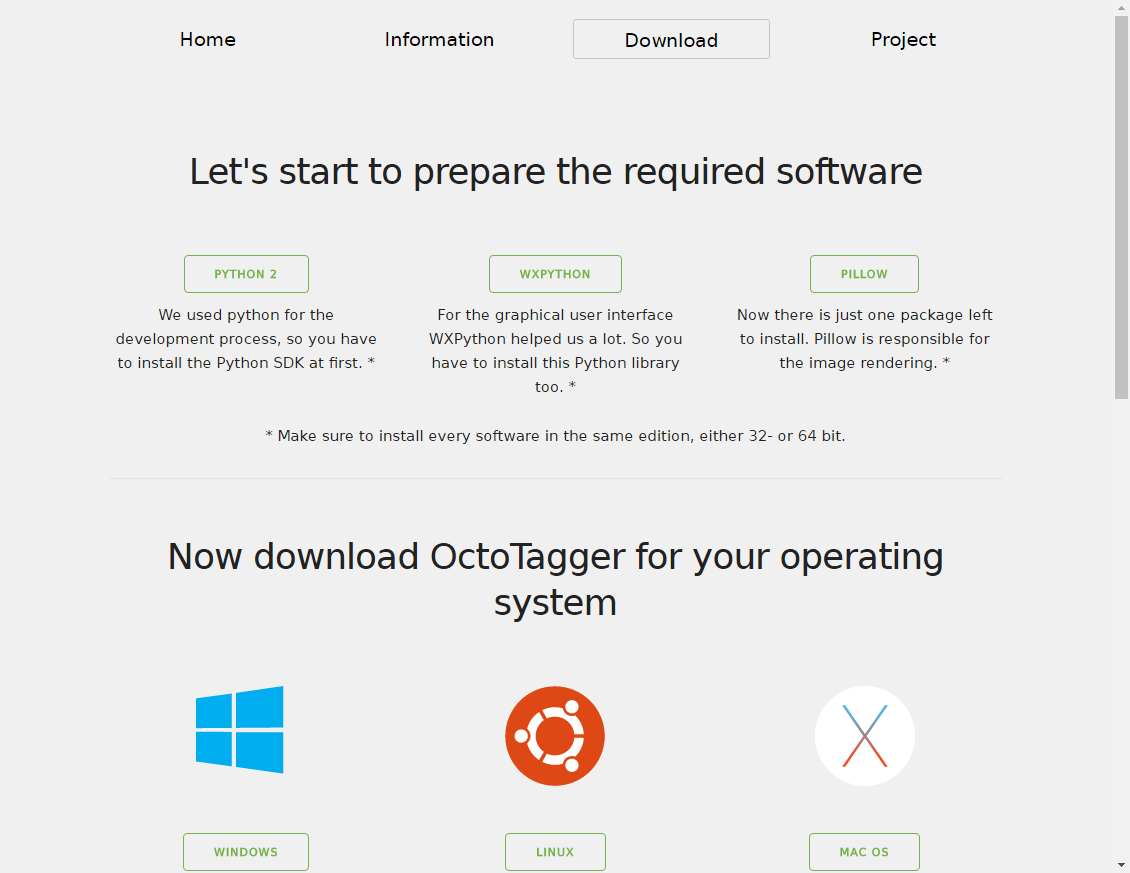
\includegraphics[scale=0.35]{images/download_full.png}
\end{center}

This page contains every available download and instructions for the installation. It's built like a step by step tutorial to guide the user through the entire process.

At first the user has to install the required software. The buttons on the top link to the developer website of the software. When a button is hovered, a dropdown menu shows up and offers further information. When the button is clicked the download site opens in a new tab.
 
The second step describes the installation of OctoTagger itself. These download buttons also provide hover functionality, which offers links to the installation guide. By clicking the download button the download starts directly. Windows user also have to install additional software to be able to use OctoTagger, which is described in the installation guide. 

In addition the user also has the possibility to download only Pywinlink, which is a service allowing symbolic links without the need of administrator rights. This service is required for OctoTagger on Windows, but is already included into the download above.

In the last step the user can download the user manual as PDF.

On the bottom of the page a link to the project Git repository can also be found.

\subsubsection{Project page}

\begin{center}
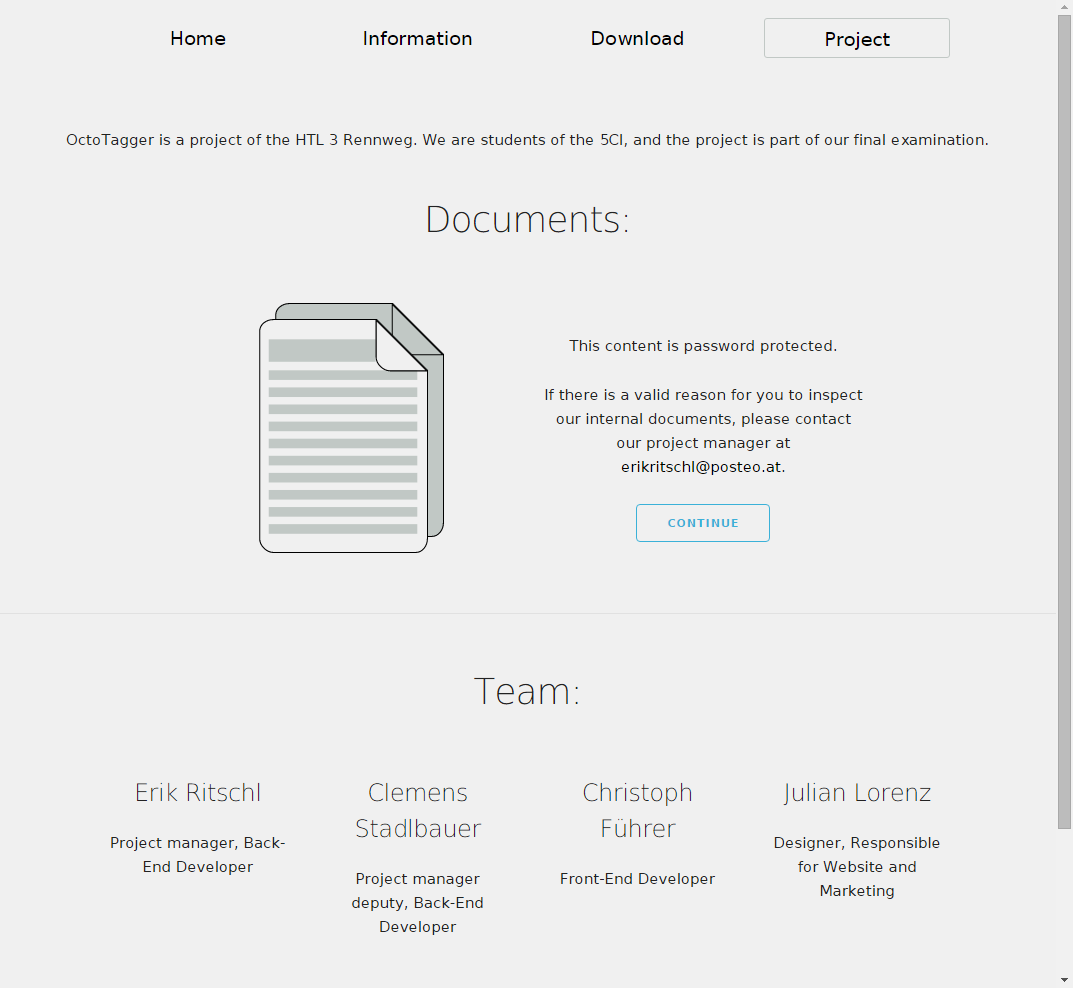
\includegraphics[scale=0.35]{images/project_full.png}
\end{center}

On this page information about the team, contact details and a link to some of our internal documents are brought together. 

\subsection{Used Tools and Technologies}

The following software, tools and frameworks helped us a lot at developing the website. Large and complex frameworks have completely been avoided to reduce loading times.


\subsubsection{Skeleton (Responsive CSS Framework)}
\label{sec:Skeleton}

Skeleton (http://getskeleton.com) is a framework which supports you with responsive development. Its source code consists of extremely few lines of code, making it great for small websites. Because of that Skeleton requires a lot of work of the developer and is basically only capable of managing the responsive grid system. It's everything you would need for responsive design, but nothing more.

\subsubsection{Adobe Illustrator}

This vector graphics editor was used for the creation of the images. 

\subsubsection{Sublime Text (Editor)}

\subsubsection{Operation System detection}
\label{sec:OSdetection}

Javascript allows the developer to check the user's operating system within just one line of code.



\subsection{Hosting}

The server is operated by the cloud provider Cloudatcost. This provider was chosen due to positive experiences in past projects and the possibility to buy a server for all time by a one-time payment. In addition, the price of 35 \$ for a simple web server is affordable for our project team. 

The server provides more then enough processing power for our needs and it's possible to install every available software on it thanks to command line control.

Namecheap was our choice concerning the purchase of the domain. This made another 8.88 \$ to use octotagger.co for one year.
% TODO like module

\section{Quality Management}
\def\kapitelautor{Julian Lorenz}
% TODO
